\chapter{Matrix Algebra}\label{chap:ch9}

In the previous chapters, we explored concepts like linear equations, echelon forms, row reductions, linear independence, vector equations, and matrix equations. Now, to take our problem-solving skills to the next level, we need to dive into matrix algebra. Matrix operations allow us to handle complex systems more efficiently, building on the foundations we've established. The tools and techniques in this chapter will streamline the way we work with multiple matrices and lead us toward deeper insights, including key ideas like the Invertible Matrix Theorem.

\section{Matrix Arithmetic}
Matrix arithmetic like adding, subtracting, scaling, and multiplying let you combine and manipulate matrices in simple ways. These operations are the building blocks for more complex matrix manipulations, like solving systems of equations and finding inverses.


\subsection*{Addition and Scalar Multiplication}
We begin with the definition of matrix addition.

\begin{definition}{Matrix Addition}
    Let $A$ and $B$ be $m \times n$ matrices. The \textbf{sum} of $A$ and $B$, denoted $A + B$, is the $m \times n$ matrix whose entries are obtained by adding the corresponding entries of $A$ and $B$.

    Given matrices

    $$
    A=\left[\begin{array}{cccc}
    a_{11} & a_{12} & \cdots & a_{1 n} \\
    a_{21} & a_{22} & \cdots & a_{2 n} \\
    \vdots & \vdots & \vdots & \vdots \\
    a_{m 1} & a_{m 2} & \cdots & a_{m n}
    \end{array}\right], \quad B=\left[\begin{array}{cccc}
    b_{11} & b_{12} & \cdots & b_{1 n} \\
    b_{21} & b_{22} & \cdots & b_{2 n} \\
    \vdots & \vdots & \vdots & \vdots \\
    b_{m 1} & b_{m 2} & \cdots & b_{m n}
    \end{array}\right]
    $$

    both of the same dimension $m \times n$, the sum $A+B$ is thus defined as

    $$
    A+B=\left[\begin{array}{cccc}
    a_{11}+b_{11} & a_{12}+b_{12} & \cdots & a_{1 n}+b_{1 n} \\
    a_{21}+b_{21} & a_{22}+b_{22} & \cdots & a_{2 n}+b_{2 n} \\
    \vdots & \vdots & \vdots & \vdots \\
    a_{m 1}+b_{m 1} & a_{m 2}+b_{m 2} & \cdots & a_{m n}+b_{m n}
    \end{array}\right]
    $$
\end{definition}

\begin{remark}
    Similar considerations apply for substraction of matrices, although not mentioned here explicitly.
\end{remark}

Next is the definition of scalar-matrix multiplication. \newpage

\begin{definition}{Scalar-Matrix Multiplication}
    Let $A$ be an $m \times n$ matrix and $c$ be a scalar. The \textbf{product} of $c$ and $A$, denoted $cA$, is the $m \times n$ matrix whose entries are obtained by multiplying each entry of $A$ by $c$, and is thus defined as

    $$
    c A=\left[\begin{array}{cccc}
    a_{11} & a_{12} & \cdots & a_{1 n} \\
    a_{21} & a_{22} & \cdots & a_{2 n} \\
    \vdots & \vdots & \vdots & \vdots \\
    a_{m 1} & a_{m 2} & \cdots & a_{m n}
    \end{array}\right] = \left[\begin{array}{cccc}
    c a_{11} & c a_{12} & \cdots & c a_{1 n} \\
    c a_{21} & c a_{22} & \cdots & c a_{2 n} \\
    \vdots & \vdots & \vdots & \vdots \\
    c a_{m 1} & c a_{m 2} & \cdots & c a_{m n}
    \end{array}\right]
    $$
    
\end{definition}

 \begin{example}
    Given matrices
    \[
A=\left[\begin{array}{ccc}
-5 & 2 & 0 \\
7 & -3 & 4 \\
-1 & 3 & 2
\end{array}\right] , \quad
B=\left[\begin{array}{ccc}
0 & -1 & 8 \\
6 & -14 & 2 \\
9 & 5 & 1
\end{array}\right]
\]
    find the sum $A + B$ and the product $3A$.
 \end{example}

\begin{solution}
    The sum $A + B$ is obtained by adding the corresponding entries of $A$ and $B$:
\begin{align*}
\begin{split}
A+B & =\left[\begin{array}{ccc}
-5 & 2 & 0 \\
7 & -3 & 4 \\
-1 & 3 & 2
\end{array}\right]+\left[\begin{array}{ccc}
0 & -1 & 8 \\
6 & -14 & 2 \\
9 & 5 & 1
\end{array}\right] \\
& =\left[\begin{array}{ccc}
(-5)+(0) & (2)+(-1) & (0)+(8) \\
(7)+(6) & (-3)+(-14) & (4)+(2) \\
(-1)+(9) & (3)+(5) & (2)+(1)
\end{array}\right] \\
& =\left[\begin{array}{ccc}
-5 & 1 & 8 \\
13 & -17 & 6 \\
8 & 8 & 3
\end{array}\right]
\end{split}
\intertext{The product $3A$ is obtained by multiplying each entry of $A$ by $3$:}
\begin{split}
3A & = 3 \left[\begin{array}{ccc}
-5 & 2 & 0 \\
7 & -3 & 4 \\
-1 & 3 & 2
\end{array}\right] \\
& = \left[\begin{array}{ccc}
3(-5) & 3(2) & 3(0) \\
3(7) & 3(-3) & 3(4) \\
3(-1) & 3(3) & 3(2)
\end{array}\right] \\
& = \left[\begin{array}{ccc}
-15 & 6 & 0 \\
21 & -9 & 12 \\
-3 & 9 & 6
\end{array}\right]
\end{split}
\end{align*}
\end{solution}

\begin{example}
Given $A$ and $B$ below, find $3A-2B$.
\[
    A=\left[\begin{array}{lll}
    1 & -2 & 5 \\
    0 & -3 & 9 \\
    4 & -6 & 7
    \end{array}\right], B=\left[\begin{array}{ccc}
    5 & 0 & -11 \\
    3 & -5 & 1 \\
    -1 & -9 & 0
    \end{array}\right]
    \]
    
\end{example}

\begin{solution}
    We compute:

    \[
\begin{aligned}
3 A-2 B & =\left[\begin{array}{ccc}
3 & -6 & 15 \\
0 & -9 & 27 \\
12 & -18 & 21
\end{array}\right]-\left[\begin{array}{ccc}
10 & 0 & -22 \\
6 & -10 & 2 \\
-2 & -18 & 0
\end{array}\right] \\
& =\left[\begin{array}{ccc}
-7 & -6 & 37 \\
-6 & 1 & 25 \\
14 & 0 & 21
\end{array}\right]
\end{aligned}
\]
\end{solution}

Before moving on to matrix multiplication, we need to state some basic algebraic properties of matrix addition and scalar multiplication.

\begin{theorem}

    Let $A$, $B$, $C$ be matrices of the same size and let $\alpha$, $\beta$ be scalars. Then
    \begin{enumerate}[(a)]
        \item $A+B=B+A$
        \item $(A+B)+C=A+(B+C)$
        \item $A+0=A$
        \item $\alpha(A+B)=\alpha A+\alpha B$
        \item $(\alpha+\beta) A=\alpha A+\beta A$
        \item $\alpha(\beta A)=(\alpha \beta) A$
    \end{enumerate}
\end{theorem}
\subsection*{Matrix Multiplication}
Matrix multiplication is a bit more complex than addition and scalar multiplication. The product of two matrices is defined only when the number of columns in the first matrix is equal to the number of rows in the second matrix. The product of two matrices $A$ and $B$ is a new matrix $C$ whose entries are determined by the dot product of the rows of $A$ and the columns of $B$. Note that $\vect{x}$ is a column vector.

Let \(B\) be an \(n \times p\) matrix and \(A\) be an \(m \times n\) matrix. If \(\vect{x} \in \mathbb{R}^p\), then multiplying \(B\) by \(\vect{x}\) produces a new vector \(B\vect{x}\) in \(\mathbb{R}^n\). Once we have this result, we can further multiply it by \(A\), giving us \(A(B\vect{x})\), which is a vector in \(\mathbb{R}^m\).

Thus, for any vector \(\vect{x}\) in \(\mathbb{R}^p\), this process produces a corresponding vector in \(\mathbb{R}^m\). This two-step operation—first multiplying by \(B\) and then by \(A\)—is referred to as the composition of \(A\) and \(B\), and is usually written as \(AB\). Therefore, we have:

\[
(AB)\vect{x} = A(B\vect{x})
\]

To compute the matrix resulting from this composition, we multiply \(A\) by \(B\) directly, following the rules of matrix multiplication. The result is a matrix \(C = AB\), where each entry of \(C\) is determined by the interactions between the rows of \(A\) and the columns of \(B\).

In essence, \(C\) represents the matrix that captures the combined effect of applying both \(B\) and \(A\) to any vector \(\vect{x} \in \mathbb{R}^p\), without needing to break it down into intermediate steps.

\begin{definition}
    For $A \in \mathbb{R}^{m \times n}$ and $B \in \mathbb{R}^{n \times p}$, with $B=\left[\begin{array}{lll}\vect{b_1} & \vect{b_2} \cdots & \vect{b_p}\end{array}\right]$, we define the product $A B$ by the formula

\[
A B=\left[\begin{array}{llll}
A \vect{b_1} & A \vect{b_2} & \cdots & A \vect{b_p}
\end{array}\right]
\]

\end{definition}

The product $AB$ is defined only when the number of columns of $A$ equals the number of rows of $B$. The following diagram is useful for remembering this:


\[
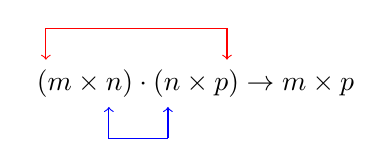
\begin{tikzpicture}
    % The matrix multiplication expression
    \node at (0,0) {\((m \times n) \cdot (n \times p) \rightarrow m \times p\)};
    
    % Red bidirectional U-shaped arrow on top
    \draw[red,<-] (-1.9,0.3) -- (-1.9,0.7) -- (0.4,0.7);
    \draw[red,->] (0.4,0.7) -- (0.4,0.3);
    
    % Blue bidirectional U-shaped arrow on the bottom
    \draw[blue,<-] (-1.1,-0.3) -- (-1.1,-0.7) -- (-0.35,-0.7);
    \draw[blue,->] (-0.35,-0.7) -- (-0.35,-0.3);
\end{tikzpicture}
\]

The diagram shows that the number of columns in the first matrix must equal the number of rows in the second matrix (the \textcolor{blue}{blue arrow}). The result is a new matrix with the number of rows from the first matrix and the number of columns from the second matrix (the \textcolor{red}{red arrow}).

\begin{example}
    For $A$ and $B$ below compute $AB$ and $BA$.

    \[
    A=\left[\begin{array}{lll}
    1 & 2 & -2 \\
    1 & 1 & -3
    \end{array}\right], \quad B=\left[\begin{array}{cccc}
    -4 & 2 & 4 & -4 \\
    -1 & -5 & -3 & 3 \\
    -4 & -4 & -3 & -1
    \end{array}\right]
    \]
    
\end{example}

\begin{solution}
    First $A B=\left[\begin{array}{llll}A \vect{b_1} & A \vect{b_2} & A \vect{b_3} & A \vect{b_4}\end{array}\right]$ :

\[
\begin{aligned}
& A B=\left[\begin{array}{lll}
1 & 2 & -2 \\
1 & 1 & -3
\end{array}\right]\left[\begin{array}{cccc}
-4 & 2 & 4 & -4 \\
-1 & -5 & -3 & 3 \\
-4 & -4 & -3 & -1
\end{array}\right] \\
& = \vcenter{\hbox{\begin{tikzpicture}
    \matrix (m1) [matrix of math nodes,left delimiter={[}] {
    2 & \quad \text{Row 1 of $A$ and Column 1 of $B$} \\
    7 & \quad \text{Row 2 of $A$ and Column 1 of $B$} \\
    };
    \draw[headercolor,thick] (m1-1-1.north west) rectangle (m1-2-1.south east);
\end{tikzpicture}}} \\
& = \vcenter{\hbox{\begin{tikzpicture}
    \matrix (m2) [matrix of math nodes,left delimiter={[}] {
    2 & 0 & \quad \text{Row 1 of $A$ and Column 2 of $B$} \\
    7 & 9 & \quad \text{Row 2 of $A$ and Column 2 of $B$} \\
    };
    \draw[headercolor,thick] (m2-1-2.north west) rectangle (m2-2-2.south east);
\end{tikzpicture}}} \\
& = \vcenter{\hbox{\begin{tikzpicture}
    \matrix (m3) [matrix of math nodes,left delimiter={[}] {
    2 & 0 & 4 & \quad \text{Row 1 of $A$ and Column 3 of $B$} \\
    7 & 9 & 10 & \quad \text{Row 2 of $A$ and Column 3 of $B$} \\
    };
    \draw[headercolor,thick] (m3-1-3.north west) rectangle (m3-2-3.south east);
\end{tikzpicture}}} \\
& = \vcenter{\hbox{\begin{tikzpicture}
    \matrix (m4) [matrix of math nodes,left delimiter={[}] {
    2 & 0 & 4 & 4 & \quad \text{Row 1 of $A$ and Column 4 of $B$} \\
    7 & 9 & 10 & 2 & \quad \text{Row 2 of $A$ and Column 4 of $B$} \\
    };
    \draw[headercolor,thick] (m4-1-4.north west) rectangle (m4-2-4.south east);
\end{tikzpicture}}} \\
& = \vcenter{\hbox{\begin{tikzpicture}
    \matrix (m4) [matrix of math nodes,left delimiter={[}, right delimiter={]}] {
    2 & 0 & 4 & 4 \\
    7 & 9 & 10 & 2 \\
    };
\end{tikzpicture}}}
\end{aligned}
\]

On the other hand, $B A$ is not defined! $B$ has 4 columns and $A$ has 2 rows. Thus, the number of columns in $B$ is not equal to the number of rows in $A$. \end{solution}

\begin{example}
    Example Compute the matrix $A B$, where

\[
A=\left[\begin{array}{ll}
1 & 2 \\
2 & 3 \\
3 & 4
\end{array}\right], \quad \text { and } B=\left[\begin{array}{cc}
2 & -1 \\
3 & 1
\end{array}\right]
\]

\end{example}

\begin{solution}
    By the definition of multiplication given above,

\[
\begin{aligned}
A B & =\left[A\left[\begin{array}{l}
2 \\
3
\end{array}\right] A\left[\begin{array}{c}
-1 \\
1
\end{array}\right]\right] \\
& \left.=\left[\begin{array}{ll}
1 & 2 \\
2 & 3 \\
3 & 4
\end{array}\right]\left[\begin{array}{l}
2 \\
3
\end{array}\right]\left[\begin{array}{ll}
1 & 2 \\
2 & 3 \\
3 & 4
\end{array}\right]\left[\begin{array}{c}
-1 \\
1
\end{array}\right]\right] \\
& =\left[\left[\begin{array}{l}
1 \cdot 2+2 \cdot 3 \\
2 \cdot 2+3 \cdot 3 \\
3 \cdot 2+4 \cdot 3
\end{array}\right]\left[\begin{array}{l}
1 \cdot(-1)+2 \cdot 1 \\
2 \cdot(-1)+3 \cdot 1 \\
3 \cdot(-1)+4 \cdot 1
\end{array}\right]\right] \\
& =\left[\begin{array}{cc}
8 & 1 \\
13 & 1 \\
18 & 1
\end{array}\right]
\end{aligned}
\]
\end{solution}

\begin{example} If $A$ is $3 \times 5$ and $B$ is $5 \times 2$, what are the sizes of $A B$ and $B A$ (assuming they are defined)?
\end{example}

\begin{solution}
    \begin{itemize}
        \item The product $A B$ is defined since the number of columns of $A$ matches the number of rows of $B$ (5). The resulting matrix $A B$ is a $3 \times 2$ matrix.
        \item The product $B A$ is not defined, since the number of columns of $B$ (2) does not match the number of rows of $A$ (3).
    \end{itemize}
\end{solution}

The next example illustrate that even if both $AB$ and $BA$ are defined, they are not necessarily equal.

\begin{example}
    For $A = \left[\begin{array}{rrr}
        -4 & 4 & 3 \\
        3 & -3 & -1 \\
        -2 & -1 & 1
        \end{array}\right] $ and $B = \left[\begin{array}{rrr}
            -1 & -1 & 0 \\
            -3 & 0 & -2 \\
            -2 & 1 & -2
            \end{array}\right]$ compute $AB$ and $BA$.

\end{example}

\begin{solution}
    First $AB$:

    \[
    \begin{aligned}
    A B &=\left[\begin{array}{rrr}
    -4 & 4 & 3 \\
    3 & -3 & -1 \\
    -2 & -1 & 1
    \end{array}\right]\left[\begin{array}{rrr}
    -1 & -1 & 0 \\
    -3 & 0 & -2 \\
    -2 & 1 & -2
    \end{array}\right] \\
    & =\left[\begin{array}{c}
    -14 \\
    8 \\
    3
    \end{array}\right. \\
    & =\left[\begin{array}{rr}
    -14 & 7 \\
    8 & -4 \\
    3 & 3
    \end{array}\right. \\
    & =\left[\begin{array}{rrr}
    -14 & 7 & -14 \\
    8 & -4 & 8 \\
    3 & 3 & 0
    \end{array}\right]
    \end{aligned}
    \]

    Next $BA$:
    \[
    \begin{aligned}
    B A & =\left[\begin{array}{rrr}
    -1 & -1 & 0 \\
    -3 & 0 & -2 \\
    -2 & 1 & -2
    \end{array}\right]\left[\begin{array}{rrr}
    -4 & 4 & 3 \\
    3 & -3 & -1 \\
    -2 & -1 & 1
    \end{array}\right] \\
    & =\left[\begin{array}{rrr}
    1 \\
    16 & \\
    15
    \end{array}\right. \\
    & =\left[\begin{array}{rrr}
    1 & -1 \\
    16 & -10 \\
    15 & -9
    \end{array}\right. \\
    & =\left[\begin{array}{rrr}
    1 & -1 & -2 \\
    16 & -10 & -11 \\
    15 & -9 & -9
    \end{array}\right]
    \end{aligned}
    \]

    We see that $AB \neq BA$. \end{solution}

    In regular arithmetic the multiplicative identity is 1. In matrix algebra, the multiplicative identity is the identity matrix, denoted by $I$. The identity matrix is a \textit{square} matrix with 1s on the diagonal and 0s elsewhere. The size of the identity matrix is determined by the context, and is usually clear from the context. For example, $I_2$ is a $2 \times 2$ identity matrix, and $I_3$ is a $3 \times 3$ identity matrix and in general $I_n \in \mathbb{R}^{n \times n}$ is an $n \times n$ identity matrix:

    $$
    I_n=\left[\begin{array}{ccccc}
    1 & 0 & 0 & \cdots & 0 \\
    0 & 1 & 0 & \cdots & 0 \\
    \vdots & \vdots & \vdots & \cdots & \vdots \\
    0 & 0 & 0 & \cdots & 1
    \end{array}\right]
    $$

    We can now state the following theorem.

    \begin{theorem}
        Let $A, B, C$ be matrices, of appropriate dimensions, and let $\alpha$ be a scalar. Then
\begin{enumerate}[(a)]
    \item $A(BC) = (AB)C$
    \item $A(B + C) = AB + AC$
    \item $(B + C)A = BA + CA$
    \item $\alpha(AB) = (\alpha A)B = A(\alpha B)$
    \item $I_n A = AI_n = A$
\end{enumerate}
\end{theorem}

We conclude this section by looking at the $k$th power of a matrix. \newpage

\begin{definition}
    Let $A$ be a square matrix, i.e. $ A \in \mathbb{R}^{n \times n}$. The $k$th power of $A$, denoted $A^k$, is defined as the product of $A$ with itself $k$ times. That is,

    $$
    A^k=\underbrace{ AAA \cdot \cdots A}_{k \text { times }}
    $$

    where $A$ appears $k$ times on the right-hand side.
\end{definition}

\begin{example}
    Compute $A^3$ if
    \[
    A=\left[\begin{array}{rr}
    -2 & 3 \\
    1 & 0
    \end{array}\right]
    \]
\end{example}

\begin{solution}

    Compute $A^2$ :

    \[
    A^2=\left[\begin{array}{rr}
    -2 & 3 \\
    1 & 0
    \end{array}\right]\left[\begin{array}{rr}
    -2 & 3 \\
    1 & 0
    \end{array}\right]=\left[\begin{array}{rr}
    7 & -6 \\
    -2 & 3
    \end{array}\right]
    \]

    And then $A^3$ :

    \[
    \begin{aligned}
    A^3=A^2 A & =\left[\begin{array}{rr}
    7 & -6 \\
    -2 & 3
    \end{array}\right]\left[\begin{array}{rr}
    -2 & 3 \\
    1 & 0
    \end{array}\right] \\
    & =\left[\begin{array}{rr}
    -20 & 21 \\
    7 & -6
    \end{array}\right]
    \end{aligned}
    \]

    We could also do:

    \[
    A^3=A A^2=\left[\begin{array}{rr}
    -2 & 3 \\
    1 & 0
    \end{array}\right]\left[\begin{array}{rr}
    7 & -6 \\
    -2 & 3
    \end{array}\right]=\left[\begin{array}{rr}
    -20 & 21 \\
    7 & -6
    \end{array}\right]
    \]

\end{solution}

\section{Matrix Transpose}
We begin with the definition of the transpose of a matrix.

\begin{definition}
    Given a matrix $A \in \mathbb{R}^{m \times n}$, the transpose of $A$ is the matrix $A^T$ whose $i$th column is the $i$th row of $A$.
\end{definition}

If $A$ is $m \times n$ then $A^T$ is $n \times m$. For example, if

\[
A=\left[\begin{array}{rrrrr}
0 & -1 & 8 & -7 & -4 \\
-4 & 6 & -10 & -9 & 6 \\
9 & 5 & -2 & -3 & 5 \\
-8 & 8 & 4 & 7 & 7
\end{array}\right]
\]

then

\[
A^T=\left[\begin{array}{rrrr}
0 & -4 & 9 & -8 \\
-1 & 6 & 5 & 8 \\
8 & -10 & -2 & 4 \\
-7 & -9 & -3 & 7 \\
-4 & 6 & 5 & 7
\end{array}\right]
\]

\begin{example} Compute $(AB)^T$ and $B^T A^T$ if

\[
A=\left[\begin{array}{rrr}
-2 & 1 & 0 \\
3 & -1 & -3
\end{array}\right], \quad B=\left[\begin{array}{rrr}
-2 & 1 & 2 \\
-1 & -2 & 0 \\
0 & 0 & -1
\end{array}\right].
\]
\end{example}

\begin{solution}
    First, compute $(AB)^T$:

    \[
    \begin{aligned}
    A B &=\left[\begin{array}{rrr}
    -2 & 1 & 0 \\
    3 & -1 & -3
    \end{array}\right]\left[\begin{array}{rrr}
    -2 & 1 & 2 \\
    -1 & -2 & 0 \\
    0 & 0 & -1
    \end{array}\right] \\
    &=\left[\begin{array}{rrr}
        3 & -4 & -4 \\
        -5 & 5 & 9
        \end{array}\right]
    \end{aligned}
    \]

    and then $(AB)^T$:

    \[
    \begin{aligned}
    (A B)^{T} &=\left[\begin{array}{rrr}
        3 & -4 & -4 \\
        -5 & 5 & 9
        \end{array}\right]^{T} \\
    &=\left[\begin{array}{rr}
        3 & -5 \\
        -4 & 5 \\
        -4 & 9
        \end{array}\right]
    \end{aligned}
    \]

    Next, compute $B^T A^T$:

    \[
    \begin{aligned}
    B^{T} A^{T} &=\left[\begin{array}{rrr}
        -2 & -1 & 0 \\
        1 & -2 & 0 \\
        2 & 0 & -1
        \end{array}\right]\left[\begin{array}{rr}
        -2 & 3 \\
        1 & -1 \\
        0 & -3
        \end{array}\right] \\
    &=\left[\begin{array}{rr}
    3 & -5 \\
    -4 & 5 \\
    -4 & 9
    \end{array}\right]
    \end{aligned}
    \]

    We see that $(AB)^T = B^T A^T$. \end{solution}

The following theorem summarises the properties of the transpose of a matrix.

\begin{theorem}
    Let $A$ and $B$ be matrices of appropriate dimensions and let $\alpha$ be a scalar. Then
    \begin{enumerate}[(a)]
        \item $(A^T)^T = A$
        \item $(A + B)^T = A^T + B^T$
        \item $(\alpha A)^T = \alpha A^T$
        \item $(AB)^T = B^T A^T$
    \end{enumerate}
\end{theorem}

A consequence of property (4) is that
\[
\left(A_1 A_2 \ldots A_k\right)^T=A_k^T A_{k-1}^T \cdots A_2^T A_1^T
\]

and as a special case

\[
\left(A^k\right)^T=\left(A^T\right)^k
\]

\section{Invertible Matrices}
The inverse of a square matrix \( A \in \mathbb{R}^{n \times n} \) extends the concept of the reciprocal for a nonzero real number \( a \in \mathbb{R} \). More precisely, the inverse of a non-zero number \( a \in \mathbb{R} \) is the unique number \( c \in \mathbb{R} \) such that \( a c = c a = 1 \). The inverse of \( a \neq 0 \), typically written as \( a^{-1} = \frac{1}{a} \), enables solving the equation \( a x = b \):

\[
a x = b \Rightarrow a^{-1} a x = a^{-1} b \Rightarrow x = a^{-1} b.
\]

This concept extends to square matrices, where the inverse of a matrix \( A \in \mathbb{R}^{n \times n} \) is a matrix \( C \in \mathbb{R}^{n \times n} \) such that \( A C = C A = I_n \), where \( I_n \) is the identity matrix of size \( n \times n \). The inverse of a matrix is denoted by \( A^{-1} \). We can now define the invertible matrix.

\begin{definition}
    A square matrix \( A \in \mathbb{R}^{n \times n} \) is invertible (or \textbf{nonsingular}) if there exists a matrix \( C \in \mathbb{R}^{n \times n} \) such that \( A C = C A = I_n \). The matrix \( C \) is called the inverse of \( A \) and is denoted by \( A^{-1} \). Thus, \( A^{-1} A = A A^{-1} = I_n \).
\end{definition}

\begin{example}
    Given $A$ and $C$ below, show that $C$ is the inverse of $A$.

    \[
    A=\left[\begin{array}{rrr}
    1 & -3 & 0 \\
    -1 & 2 & -2 \\
    -2 & 6 & 1
    \end{array}\right], \quad C=\left[\begin{array}{rrr}
    -14 & -3 & -6 \\
    -5 & -1 & -2 \\
    2 & 0 & 1
    \end{array}\right]
    \]
    \label{ex:inverse2}
\end{example}

\begin{solution}
    We need to show that $A C = C A = I_3$. First, compute $AC$:

    \[
    \begin{aligned}
    A C &=\left[\begin{array}{rrr}
    1 & -3 & 0 \\
    -1 & 2 & -2 \\
    -2 & 6 & 1
    \end{array}\right]\left[\begin{array}{rrr}
    -14 & -3 & -6 \\
    -5 & -1 & -2 \\
    2 & 0 & 1
    \end{array}\right] \\
    &=\left[\begin{array}{rrr}
    1 & 0 & 0 \\
    0 & 1 & 0 \\
    0 & 0 & 1
    \end{array}\right]=I_3
    \end{aligned}
    \]

    Next, compute $CA$:

    \[
    \begin{aligned}
    C A &=\left[\begin{array}{rrr}
    -14 & -3 & -6 \\
    -5 & -1 & -2 \\
    2 & 0 & 1
    \end{array}\right]\left[\begin{array}{rrr}
    1 & -3 & 0 \\
    -1 & 2 & -2 \\
    -2 & 6 & 1
    \end{array}\right] \\
    &=\left[\begin{array}{rrr}
    1 & 0 & 0 \\
    0 & 1 & 0 \\
    0 & 0 & 1
    \end{array}\right]=I_3
    \end{aligned}
    \]

    We see that $C=A^{-1}$ is the inverse of $A$. \end{solution}

The following theorem summarizes the relationship between the matrix inverse and matrix multiplication and matrix transpose.

\begin{theorem} Let $A$ and $B$ be invertible $n \times n$ matrices. Then:
\begin{enumerate}[(a)]
    \item $A^{-1}$ is invertible, with
    \[
    \left(A^{-1}\right)^{-1}=A
    \]
    \item The product $A B$ is invertible, with
    \[
    (A B)^{-1}=B^{-1} A^{-1}
    \]
    \item The transpose of $A$ is also invertible, i.e. $A^T$ is invertible, with
    \[
    \left(A^T\right)^{-1}=\left(A^{-1}\right)^T
    \]
\end{enumerate}

\end{theorem}

We will now consider how we can find the inverse of a matrix.

\subsection*{Finding the Determinant and Inverse of a $2 \times 2$ Matrix}

The inverse of a matrix is not always easy to find. However, for a $2 \times 2$ matrix, we can use a formula to find the inverse.

\begin{theorem}
    Let $A=\left[\begin{array}{ll}
    a & b \\
    c & d
    \end{array}\right]$. If $ad-bc \neq 0$, then the inverse of $A$ is given by

    \[
    A^{-1}=\frac{1}{ad-bc}\left[\begin{array}{cc}
    d & -b \\
    -c & a
    \end{array}\right]
    \]
\end{theorem}

\begin{remark}
    The quantity $ad - bc$ is called the determinant of $A$, and we write
    \[
    \text{det}(A) = |A| = ad - bc
    \]
\end{remark}

The determinant of a $2 \times 2$ matrix is a scalar quantity that provides information about the matrix. If the determinant is zero, then the matrix is not invertible. If the determinant is non-zero, then the matrix is invertible. These formulae are only valid $2 \times 2$ matrices.

\begin{example} We let

\[
A=\left[\begin{array}{ll}
1 & 2 \\
3 & 4
\end{array}\right]
\]

and compute $A^{-1}$. By the theorem, we have

\[
\begin{aligned}
A^{-1} & =\frac{1}{1 \cdot 4-2 \cdot 3}\left[\begin{array}{cc}
4 & -2 \\
-3 & 1
\end{array}\right] \\
& =-\frac{1}{2}\left[\begin{array}{cc}
4 & -2 \\
-3 & 1
\end{array}\right] \\
& =\left[\begin{array}{cc}
-2 & 1 \\
\frac{3}{2} & -\frac{1}{2}
\end{array}\right]
\end{aligned}
\]

Now we confirm that $A A^{-1}=I_2$ :

\[
\begin{aligned}
A A^{-1} & =\left[\begin{array}{ll}
1 & 2 \\
3 & 4
\end{array}\right]\left[\begin{array}{cc}
-2 & 1 \\
\frac{3}{2} & -\frac{1}{2}
\end{array}\right] \\
& =\left[\begin{array}{ll}
1(-2)+2\left(\frac{3}{2}\right) & 1(1)+2\left(-\frac{1}{2}\right) \\
3(-2)+4\left(\frac{3}{2}\right) & 3(1)+4\left(-\frac{1}{2}\right)
\end{array}\right] \\
& =\left[\begin{array}{ll}
-2+3 & 1-1 \\
-6+6 & 3-2
\end{array}\right] \\
& =\left[\begin{array}{ll}
1 & 0 \\
0 & 1
\end{array}\right]
\end{aligned}
\]
\label{ex:inverse}
\end{example}

\begin{example} Find the inverse of $A=\left[\begin{array}{cc}1 & 3 \\ -1 & -2\end{array}\right]$ if it exists.
    
\end{example}

\begin{solution}
    We first compute the determinant of $A$:

    \[
    \text{det}(A)=1(-2)-3(-1)=(-2)+3=1
    \]

    Since the determinant is non-zero, the inverse of $A$ exists. By the formula, we have

    \[
    \begin{aligned}
    A^{-1} & =\frac{1}{1}\left[\begin{array}{cc}-2 & -3 \\ 1 & 1\end{array}\right]
    \end{aligned}
    \]

    We can confirm that $A A^{-1}=I_2$:

    \[
        A A^{-1}=\left[\begin{array}{cc}
    1 & 3 \\
    -1 & -2
    \end{array}\right]\left[\begin{array}{cc}
    -2 & -3 \\
    1 & 1
    \end{array}\right]=\left[\begin{array}{ll}
    1 & 0 \\
    0 & 1
    \end{array}\right] =I_2
    \]

\end{solution}

For larger matrices, we need to use other methods to find the inverse.

\subsection*{Finding the Inverse of a $n \times n$ Matrix}
An \textbf{elementary matrix} is a matrix that is obtained by performing a single elementary row operation (replacement, swap, or scaling) on an identity matrix. For example, the matrix

\[
E_1=\left[\begin{array}{ccc}
1 & 0 & 0 \\
0 & 1 & 0 \\
-2 & 0 & 1
\end{array}\right]
\]

is an elementary matrix since it is obtained from $I_3$ via the single elementary row operation $r_3 \mapsto r_3-2 r_1$.

\begin{example}

Let $A$ be a general $3 \times 3$ matrix

\[
A=\left[\begin{array}{lll}
a & b & c \\
d & e & f \\
g & h & i
\end{array}\right]
\]

and we let $E_1, E_2$, and $E_3$ be the elementary matrices

\[
E_1=\left[\begin{array}{ccc}
1 & 0 & 0 \\
0 & 1 & 0 \\
-2 & 0 & 1
\end{array}\right], \quad E_2=\left[\begin{array}{lll}
1 & 0 & 0 \\
0 & 0 & 1 \\
0 & 1 & 0
\end{array}\right], \quad \text { and } \quad E_3=\left[\begin{array}{lll}
1 & 0 & 0 \\
0 & 3 & 0 \\
0 & 0 & 1
\end{array}\right]
\]
\end{example}

Notice, then, that $E_1$ corresponds to $r_3 \mapsto r_3-2 r_1, E_2$ corresponds to $r_2 \longleftrightarrow r_3$, and $E_3$ corresponds to $r_2 \mapsto 3 r_2$. We also have the following products:

\[
E_1 A=\left[\begin{array}{ccc}
a & b & c \\
d & e & f \\
g-2 a & h-2 b & i-2 c
\end{array}\right], \quad E_2 A=\left[\begin{array}{ccc}
a & b & c \\
g & h & i \\
d & e & f
\end{array}\right], \quad \text { and } \quad E_3 A=\left[\begin{array}{ccc}
a & b & c \\
3 d & 3 e & 3 f \\
g & h & i
\end{array}\right] .
\]


Notice that $E_1 A$ is the matrix obtained by performing the row operation $r_3 \mapsto r_3-2 r_1$ on $A$. In general, multiplying $A$ on the left by an elementary matrix is the same as performing the corresponding row operation on $A$. We can also represent a sequence of row operations by multiplication of several elementary matrices. For example,

\[
E_2 E_1 A=\left[\begin{array}{ccc}
a & b & c \\
g-2 a & h-2 b & i-2 c \\
d & e & f
\end{array}\right]
\]

corresponds to performing $r_3 \mapsto r_3-2 r_1$ followed by $r_2 \longleftrightarrow r_3$ on the matrix $A$.
As we have observed before, row operations are reversible. It follows that elementary matrices are also invertible. This leads to the following theorem.

\begin{theorem}
    An $n \times n$ matrix $A$ is invertible if and only if $A$ is row equivalent to $I_n$. In this case, any sequence of elementary row operations that reduces $A$ to $I_n$ also transforms $I_n$ into $A^{-1}$.
\end{theorem}

This theorem leads to a nice algorithm for finding the inverse of an $n \times n$ matrix, assuming such an inverse exists.

\begin{custombox}{Algorithm for Finding the Inverse of an $n \times n$ Matrix}
    Let $A$ be an $n \times n$ matrix. To find the inverse of $A$, follow these steps:
    \begin{enumerate}
        \item Form the augmented matrix $[A | I_n]$.
        \item Perform row operations on $[A | I_n]$ to reduce $A$ to $I_n$.
        \item The matrix on the right side of the augmented matrix is $A^{-1}$.
    \end{enumerate}

    If $A$ is not invertible, then the algorithm will not be able to reduce $A$ to $I_n$.
\end{custombox}

\begin{example} Find the inverse of $A=\left[\begin{array}{rrr}1 & 0 & 3 \\ 1 & 1 & 0 \\ -2 & 0 & -7\end{array}\right]$ if it exists.    
\end{example}

\begin{solution}
    Solution. Form the augmented matrix $\left[\begin{array}{ll}A & I_3\end{array}\right]$ and row reduce:
\[
\begin{alignedat}{3}
& \left[\begin{array}{cccccc}
1 & 0 & 3 & 1 & 0 & 0 \\
1 & 1 & 0 & 0 & 1 & 0 \\
-2 & 0 & -7 & 0 & 0 & 1
\end{array}\right]
& \quad & \begin{aligned}
    r_2 &\mapsto -r_1 + r_2 \\
    r_3 &\mapsto 2 r_1 + r_3
\end{aligned}
& \quad & \left[\begin{array}{cccccc}
1 & 0 & 3 & 1 & 0 & 0 \\
0 & 1 & -3 & -1 & 1 & 0 \\
0 & 0 & -1 & 2 & 0 & 1
\end{array}\right] \\[10pt]
& & \quad & r_3 \mapsto -r_3
& \quad & \left[\begin{array}{cccccc}
1 & 0 & 3 & 1 & 0 & 0 \\
0 & 1 & -3 & -1 & 1 & 0 \\
0 & 0 & 1 & -2 & 0 & -1
\end{array}\right] \\[10pt]
& & \quad & \begin{aligned}
    r_2 &\mapsto 3 r_3 + r_2 \\
    r_1 &\mapsto -3 r_3 + r_1
\end{aligned}
& \quad & \left[\begin{array}{cccccc}
1 & 0 & 0 & 7 & 0 & 3 \\
0 & 1 & 0 & -7 & 1 & -3 \\
0 & 0 & 1 & -2 & 0 & -1
\end{array}\right]
\end{alignedat}
\]

Therefore, \(\operatorname{rref}A = I_3\), confirming that \( A \) is invertible. The inverse is
\[
A^{-1} = \left[\begin{array}{ccc}
7 & 0 & 3 \\
-7 & 1 & -3 \\
-2 & 0 & -1
\end{array}\right]
\]
Verify:
\[
AA^{-1}=\left[\begin{array}{ccc}
1 & 0 & 3 \\
1 & 1 & 0 \\
-2 & 0 & -7
\end{array}\right]\left[\begin{array}{ccc}
7 & 0 & 3 \\
-7 & 1 & -3 \\
-2 & 0 & -1
\end{array}\right]=\left[\begin{array}{lll}
1 & 0 & 0 \\
0 & 1 & 0 \\
0 & 0 & 1
\end{array}\right]
\]

\end{solution}

\begin{example}
    Find the inverse of $A=\left[\begin{array}{rrr}1 & 0 & 1 \\ 1 & 1 & -2 \\ -2 & 0 & -2\end{array}\right]$ if it exists.
\end{example}

\begin{solution}
    Form the augmented matrix $\left[\begin{array}{ll}A & I_3\end{array}\right]$ and row reduce:
\[
\begin{alignedat}{3}
& \left[\begin{array}{cccccc}
1 & 0 & 1 & 1 & 0 & 0 \\
1 & 1 & -2 & 0 & 1 & 0 \\
-2 & 0 & -2 & 0 & 0 & 1
\end{array}\right]
& \quad & \begin{aligned}
    r_2 &\mapsto -r_1 + r_2 \\
    r_3 &\mapsto 2 r_1 + r_3
\end{aligned}
& \quad & \left[\begin{array}{cccccc}
1 & 0 & 1 & 1 & 0 & 0 \\
0 & 1 & -3 & -1 & 1 & 0 \\
0 & 0 & 0 & 2 & 0 & 1
\end{array}\right]
\end{alignedat}
\]

We need not go further since the rref($A$) is not $I_3$. Therefore, A is not invertible.
\end{solution}

\begin{example}
    Find the inverse of the matrix

    \[
    A=\left[\begin{array}{lll}
        1 & 2 & 1 \\
        4 & 5 & 3 \\
        0 & 0 & 2
        \end{array}\right]
    \]
if it exists.
\end{example}

\begin{solution} (We ommit the row reduction steps for brevity.)
\[
\begin{aligned}
{\left[\begin{array}{llllll}
1 & 2 & 1 & 1 & 0 & 0 \\
4 & 5 & 3 & 0 & 1 & 0 \\
0 & 0 & 2 & 0 & 0 & 1
\end{array}\right] } & \sim\left[\begin{array}{cccccc}
1 & 2 & 1 & 1 & 0 & 0 \\
0 & -3 & -1 & -4 & 1 & 0 \\
0 & 0 & 2 & 0 & 0 & 1
\end{array}\right] \\
& \sim\left[\begin{array}{cccccc}
1 & 2 & 1 & 1 & 0 & 0 \\
0 & -3 & -1 & -4 & 1 & 0 \\
0 & 0 & 1 & 0 & 0 & \frac{1}{2}
\end{array}\right] \\
& \sim\left[\begin{array}{cccccc}
1 & 2 & 0 & 1 & 0 & -\frac{1}{2} \\
0 & -3 & 0 & -4 & 1 & \frac{1}{2} \\
0 & 0 & 1 & 0 & 0 & \frac{1}{2}
\end{array}\right] \\
& \sim\left[\begin{array}{cccccc}
1 & 2 & 0 & 1 & 0 & -\frac{1}{2} \\
0 & 1 & 0 & \frac{4}{3} & -\frac{1}{3} & -\frac{1}{6} \\
0 & 0 & 1 & 0 & 0 & \frac{1}{2}
\end{array}\right] \\
& \sim\left[\begin{array}{cccccc}
1 & 0 & 0 & -\frac{5}{3} & \frac{2}{3} & -\frac{1}{6} \\
0 & 1 & 0 & \frac{4}{3} & -\frac{1}{3} & -\frac{1}{6} \\
0 & 0 & 1 & 0 & 0 & \frac{1}{2}
\end{array}\right] .
\end{aligned}
\]

Hence

\[
A^{-1}=\left[\begin{array}{ccc}
-\frac{5}{3} & \frac{2}{3} & -\frac{1}{6} \\
\frac{4}{3} & -\frac{1}{3} & -\frac{1}{6} \\
0 & 0 & \frac{1}{2}
\end{array}\right] .
\]

\end{solution}

With the method for finding matrix inverses established, we now have a powerful tool for approaching linear systems. We will see how matrix inverses can be used to solve systems of equations efficiently, offering a straightforward way to find solutions when a matrix is invertible.

\subsection*{Solving Matrix Equations with Inverses}
Just like we can solve an equation by using the reciprocal of a non-zero number as we saw previously, we can do something similar with matrices. When a matrix \( A \) is invertible, we can use its inverse to solve matrix equations involving \( A \). This brings us to the theorem below, which shows how we can find solutions for equations like \( A \vect{x} = \vect{b} \) when \( A \) has an inverse.

\begin{theorem}
    Let \( A \) be an invertible matrix. Then the equation \( A \vect{x} = \vect{b} \) has a unique solution given by \( \vect{x} = A^{-1} \vect{b} \).
\end{theorem}

\begin{example}
We can use the inverse from example \ref{ex:inverse} to solve the linear system

\[
\begin{aligned}
x_1+2 x_2 & =5 \\
3 x_1+4 x_2 & =6 .
\end{aligned}
\]

We think of this in matrix terms as \(A \vect{x}=\vect{b}\), where

\[
A=\left[\begin{array}{ll}
1 & 2 \\
3 & 4
\end{array}\right], \quad \vect{x}=\left[\begin{array}{l}
x_1 \\
x_2
\end{array}\right], \quad \text { and } \quad \vect{b}=\left[\begin{array}{l}
5 \\
6
\end{array}\right]
\]

The theorem tells us that \(\vect{x}=A^{-1} \vect{b}\) is a solution, i.e. that

\[
\begin{aligned}
{\left[\begin{array}{l}
x_1 \\
x_2
\end{array}\right] } & =\left[\begin{array}{cc}
-2 & 1 \\
\frac{3}{2} & -\frac{1}{2}
\end{array}\right]\left[\begin{array}{l}
5 \\
6
\end{array}\right] \\
& =\left[\begin{array}{c}
-2(5)+1(6) \\
\frac{3}{2}(5)-\frac{1}{2}(6)
\end{array}\right] \\
& =\left[\begin{array}{c}
-4 \\
\frac{9}{2}
\end{array}\right]
\end{aligned}
\]
\end{example}

\begin{example} Use the result from example \ref{ex:inverse2} to solve the linear system $A \vect{x} = \vect{b}$ where

    \[A=\left[\begin{array}{rrr}1 & -3 & 0 \\ -1 & 2 & -2 \\ -2 & 6 & 1\end{array}\right], \quad \vect{b}=\left[\begin{array}{c}1 \\ -3 \\ -1\end{array}\right]\]

\end{example}

\begin{solution} We showed in example \ref{ex:inverse2} that

    \[
    A^{-1}=\left[\begin{array}{rrr}
    -14 & -3 & -6 \\
    -5 & -1 & -2 \\
    2 & 0 & 1
    \end{array}\right]
    \]

Therefore, the unique solution to the linear system $A \vect{x} = \vect{b}$ is

    \[
    A^{-1} \vect{b}=\left[\begin{array}{rrr}
    -14 & -3 & -6 \\
    -5 & -1 & -2 \\
    2 & 0 & 1
    \end{array}\right]\left[\begin{array}{c}
    1 \\
    -3 \\
    -1
    \end{array}\right]=\left[\begin{array}{l}
    1 \\
    0 \\
    1
    \end{array}\right]
    \]

Verify:

    \[
    \left[\begin{array}{rrr}
    1 & -3 & 0 \\
    -1 & 2 & -2 \\
    -2 & 6 & 1
    \end{array}\right]\left[\begin{array}{l}
    1 \\
    0 \\
    1
    \end{array}\right]=\left[\begin{array}{c}
    1 \\
    -3 \\
    -1
    \end{array}\right]
    \]
\end{solution}

We conclude this chapter with one of the most important theorems in linear algebra, The Invertible Matrix Theorem.

\section{The Invertible Matrix Theorem}

The Invertible Matrix Theorem provides a comprehensive list of equivalent statements for a square matrix to be invertible and it enables us to determine the truth value of one statement by checking the truth value of another.

\newpage

\begin{theorem}
    Let \( A \) be an \( n \times n \) matrix. The following statements are equivalent:
    \begin{enumerate}[(a)]
        \item $A$ is invertible.
        \item $A$ is row equivalent to $I_n$.
        \item $A$ has $n$ pivot positions (i.e. one for each row and column).
        \item The equation $A \vect{x}=\overline{0}$ has only the trivial solution.
        \item The columns of $A$ are linearly independent.
        \item The equation \( A \vect{x} = \vect{b} \) has a unique solution for each \( \vect{b} \in \mathbb{R}^n \).
        \item The columns of $A \operatorname{span} \mathbb{R}^n$.
        \item \( \text{det}(A) \neq 0 \).
        \item There is an $n \times n$ matrix $C$ such that $C A=I$.
        \item There is an $n \times n$ matrix $D$ such that $A D=I$.
        \item $A^T$ is invertible.
    \end{enumerate}
\end{theorem}

Note how the theorem connects the properties of a matrix to its invertibility, thus summarising the main elements of our discussion on linear systems, independence, vectors, and matrices.

\begin{example} Decide if the following matrix is invertible:

\[
A=\left[\begin{array}{lll}
2 & 2 & 2 \\
1 & 3 & 1 \\
4 & 4 & 6
\end{array}\right]
\]

\end{example}

\begin{solution}
Performing row operations, we see

\[
\begin{aligned}
A & \sim\left[\begin{array}{lll}
1 & 3 & 1 \\
2 & 2 & 2 \\
4 & 4 & 6
\end{array}\right] \\
& \sim\left[\begin{array}{ccc}
1 & 3 & 1 \\
0 & -4 & 0 \\
0 & -8 & 2
\end{array}\right] \\
& \sim\left[\begin{array}{ccc}
1 & 3 & 1 \\
0 & -4 & 0 \\
0 & 0 & 2
\end{array}\right]
\end{aligned}
\]
which has 3 pivots, so by (c) we have that $A$ is invertible.
\end{solution}

This concludes our discussion on matrices.